\documentclass[10pt]{article}
\usepackage[a4paper,margin=1.4cm,top=1.2cm,bottom=1.2cm]{geometry}
\usepackage[table]{xcolor}
\usepackage{booktabs,graphicx,amsmath,enumitem,tabularx}
\usepackage[T1]{fontenc}
\usepackage{lmodern}
\setlength{\parindent}{0pt}\setlength{\parskip}{3pt}
\setlist{nosep,leftmargin=1.2em}
\pagestyle{empty}
\definecolor{acc}{RGB}{30,80,140}
\definecolor{boxbg}{RGB}{236,242,250}
\definecolor{good}{RGB}{190,232,190}\definecolor{fair}{RGB}{252,226,160}\definecolor{poor}{RGB}{244,182,176}
\newcommand{\head}[1]{\par\smallskip{\color{acc}\large\bfseries #1}\par\vspace{1pt}}
\newcommand{\key}[1]{\par\colorbox{boxbg}{\parbox{\dimexpr\linewidth-2\fboxsep}{#1}}\par}

\begin{document}
{\color{acc}\LARGE\bfseries Amplifier and setup quality from a single readout trace}\\[2pt]
{\small Skipper-CCD output amplifiers: PA03 (130\,K, boards 101/102) and LSM production modules DM07/09/10 (180\,K) \hfill 16 November 2026}

\key{\textbf{In one sentence.} From one raw trace of one channel (about 0.2\,s of data, no image, no charge) we can now
measure separately \textbf{how much noise the setup adds}, \textbf{how good the output transistor is} (including its
gate-oxide trap density), and \textbf{whether the readout timing is settled}. Applied to 20 amplifiers on two test
stands, it shows that \textbf{our noise is limited by the setup on board 101, not by the CCD amplifiers}.}

\head{The problem}
The read noise of a skipper CCD has three sources: the readout electronics, the CCD's own output transistor, and the setup
(cabling, grounding, supplies). Until now they were separated only with full images, voltage scans, or by eye on noise
spectra, so a noisy channel could not be blamed quickly on the hardware that can be fixed (setup) or the hardware that
cannot (a defective transistor).

\head{What is new}
\begin{enumerate}
\item \textbf{A single setup number.} Remove the waveform that repeats every skip; what is left is noise. Its level
  between 200\,Hz and 1\,kHz (\textmu V/$\sqrt{\text{Hz}}$) is the band a 500-skip pixel ($\sim$16\,ms) cannot average away.
  Good $<5$, acceptable $<15$.
\item \textbf{Transistor quality from the same trace.} Shorter CDS windows are formed in software from the raw samples.
  White noise falls with the window, the transistor's 1/f noise does not, so the two separate, giving the 1/f corner and
  the oxide trap density (McWhorter model). Validated against a hardware window scan over 100 strips: within 15\,\% on two
  amplifiers, a factor 1.6 on the other two.
\item \textbf{Defect and timing flags}, also per trace: telegraph (single-trap) noise from the shape of the noise
  distribution; an unsettled signal window from the slope inside it and the CDS offset.
\end{enumerate}

\head{Main results}
\begin{minipage}[t]{0.50\linewidth}\vspace{0pt}\small
\begin{tabular}{@{}lr@{}}\toprule
setup number (0.2--1\,kHz, \textmu V/$\sqrt{\text{Hz}}$) & \\\midrule
PA03 board 101, October & \cellcolor{poor}67.6\\
PA03 board 101, November (after cabling fix) & \cellcolor{poor}34.8\\
LSM, ACM106 / 109 (typical channel) & \cellcolor{fair}5--15\\
LSM, ACM110 (quietest channels) & \cellcolor{good}2.6--4.2\\
PA03 board 102 (channels without charge) & \cellcolor{good}1.5--1.6\\\midrule
oxide trap density, all good channels & \cellcolor{good}1--2$\times10^{16}$\,eV$^{-1}$cm$^{-3}$\\
trappy transistors found & ACM109 ch1, ACM110 ch1\\\bottomrule
\end{tabular}
\end{minipage}\hfill
\begin{minipage}[t]{0.47\linewidth}\vspace{0pt}
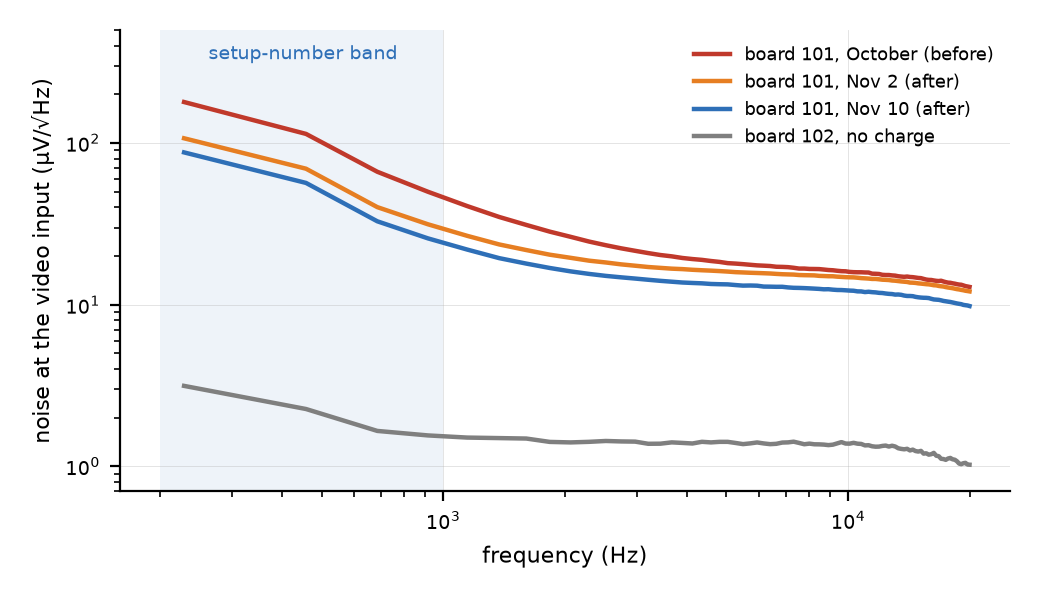
\includegraphics[width=\linewidth]{figures/raw_psd_low.png}\\[-2pt]
{\footnotesize Noise of one PA03 channel (one trace each) before and after the cabling change, against a channel
without charge. The setup number is the level in the shaded band (table: medians of 12 traces).}
\end{minipage}

\begin{itemize}
\item \textbf{Our limit is the setup, not the amplifiers.} PA03's transistors are as good as the LSM production
  modules' (same trap density, same sense node, 84--95\,fF), but board 101 carries 3--13$\times$ the LSM's slow pickup,
  and 20$\times$ that of board 102 in the same cryostat.
\item \textbf{The cabling change is quantified:} pickup halved (67.6 $\to$ 34.8), consistent with images (shared noise
  between amplifiers 25\,\% $\to$ 5\,\%).
\item \textbf{Bad channels are diagnosed}, not just flagged: ACM109 ch1 has a trappy transistor (a hardware defect),
  ACM110 ch3 picks up a 30.6\,kHz interference comb (a setup problem), PA03 101 ch2 shows extra charge (glow) and telegraph
  episodes.
\item \textbf{Readout settings:} 5--10\,\textmu s CDS windows are optimal at fixed readout time (longer costs 9--32\,\%);
  the wait after the summing-well pulse is too short on LSM board 109 and borderline on PA03.
\end{itemize}

\head{What it can be used for}
\begin{itemize}
\item \textbf{Setup debugging in minutes:} change a ground or cable, take one trace, read the setup number.
\item \textbf{Run monitoring:} one static record per channel per run; a jump in the setup number flags a new noise source.
\item \textbf{Amplifier screening and acceptance} of production modules: trap density, 1/f corner and telegraph flag per
  channel, from data already taken, separating a defective transistor (replace) from a noisy environment (fix).
\item \textbf{Comparing test stands} on one scale, and \textbf{choosing readout timing} (window length, settling waits).
\item \textbf{Physics features for the voltage-optimisation ML}, separating ``noisy settings'' from ``noisy day''.
\end{itemize}

\head{Limits and next steps}
{\small Absolute nV values rely on the design chain gain (about $\pm$5\,\%); trap densities assume the layout's follower
gain. Two measurements would close the open questions: \textbf{a board-101 trace with charge clocking off} (is the
pickup from cabling, or does it come with charge?) and \textbf{LSM images at 130\,K} (are their noisier images a 180\,K
dark-charge effect?). Details: \texttt{amp\_phys} reports and the colour-graded channel scorecard.}
\end{document}
